\section{Protoschema Matching as FrameNet Parsing}
\label{sec:lome}

\begin{figure*}
    \centering
    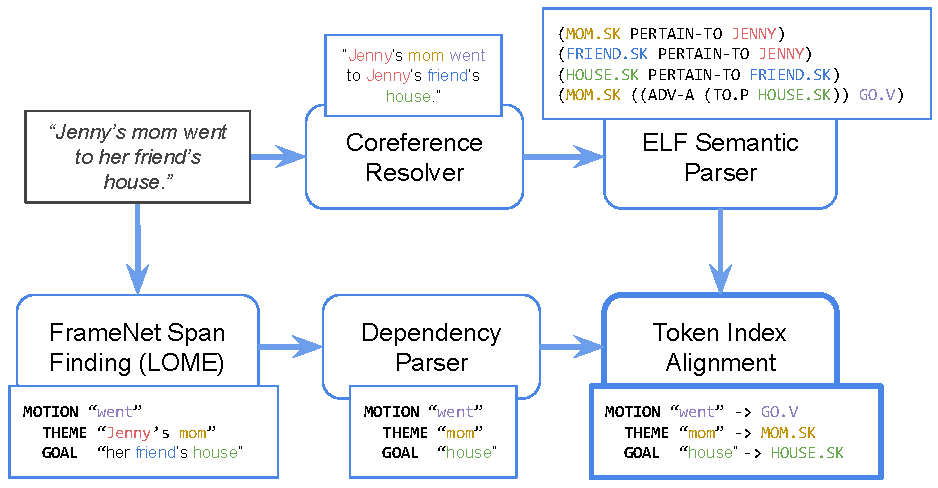
\includegraphics[width=\columnwidth]{figures/nesl/lome_architecture}
    \caption{A representation of the process by which FrameNet parsing with LOME is used for protoschema matching. The coreference resolver is provided by AllenNLP \citep{Gardner2017AllenNLP}, and the dependency parser is provided by spaCy \citep{spacy2}.}
    \label{fig:lome_architecture}
\end{figure*}

Our system's architecture, illustrated in Figure~\ref{fig:lome_architecture}, is divided into two main information pipelines: the EL track, responsible for semantic parsing, and the FrameNet track, responsible for frame identification and span selection. The information from both of these pipelines is unified into a final schematic representation at the end using token indices from the input text.

\subsection{EL Track}
To produce an EL semantic parse of the story, we first perform span mapping on the input text using the AllenNLP coreference resolver \citep{Gardner2017AllenNLP}. Co-referring token indices are saved, and story sentences are then converted into ELFs by first parsing them into ULF---an underspecified variant of EL \citep{kim2019IWCS}---and then processing the ULFs into full ELFs by converting grammatical tense information into temporal relations and scoping quantifiers. More information on the ELF parser can be found in \citep{Lawley2021LearningGE}.

Coreference resolution on the ELFs is performed by cross-referencing the token index clusters with token index tags placed on individuals in the EL parse. Co-referring individuals in the EL parse are then combined into one individual and substitutions are made throughout the parse.

\subsection{FrameNet Track}
To identify basic behavioral frames invoked by the raw text, we make use of the LOME information extraction system \citep{lome}. LOME outputs invoked frames, and text spans that fill frame roles, as \textsc{Concrete} data files. Once we extract the invoked frames and text spans, we perform a syntactic dependency parse on the input text using spaCy \citep{spacy2} and identify the first token in each span with a \texttt{NSUBJ}, \texttt{DOBJ}, or \texttt{POBJ} tag. This allows any span of text containing tokens for multiple individuals, e.g. \textit{her friend's house}, to be reduced to, e.g., \textit{house}, which will be the token used to identify the logical individual in the EL parse during the alignment phase.

\subsection{Token Index Alignment and Schema Formation}
To represent the identified FrameNet frames as EL formulas, the text spans that fill the semantic roles for each frame must first be bound to logical individuals. After the dependency parser identifies the token to cross-reference with the EL parse, the noun predicate with the same token index is retrieved from the EL parse, and the individual satisfying that predicate is identified as the bound value for the frame role.

The verb that invoked the frame is identified in a similar fashion, and a schema is created with that verb's formula from the EL parse as its header, and with the names of the FrameNet semantic roles applied to the relevant individuals as semantic types in the new schema's \texttt{Roles} section. When multiple frames are converted to schemas in this way, they may all be embedded together in a \textit{composite schema}, such as the one shown in Figure~\ref{fig:schema}, with their header formulas as steps and with each of their inner type constraints shown in the composite schema's \texttt{Roles} section for clarity. This composite schema forms our final semantic representation of the story.

%\section{Discussion}
%The goal of our representation, and of semantic story representations in general, is to enable a variety of reasoning tasks. We discuss two interesting potential applications of this representation here: question answering and event schema acquisition.